\documentclass[landscape]{article}
\usepackage{fullpage}

% To insert this map into a document, place the next three uncommented lines in 
% the preamble of the document (after your usepackage declarations). Then include
% the tikz picture as shown in lines 20:25 of this document. 
\usepackage{tikz}
\usetikzlibrary{shapes, arrows, calc, fit}
\tikzstyle{climateModel} = [rectangle, 
                            rounded corners, 
                            minimum width=6em, 
                            minimum height=3em, 
                            text centered, 
                            draw=black, 
                            fill=green!30]

\tikzstyle{iceModel}     = [rectangle, 
                            rounded corners, 
                            minimum width=6em, 
                            minimum height=3em, 
                            text centered, 
                            draw=black, 
                            fill=cyan!30]

\tikzstyle{dycore}       = [rectangle,
                            rectangle split, 
                            rectangle split parts=2,
                            minimum width=6em, 
                            text centered,
                            align=center,
                            draw=black, 
                            fill=red!30]

\tikzstyle{textBox}      = [rectangle,
                            minimum width=.25, 
                            minimum height=0.25, 
                            text centered,
                            draw=black, 
                            fill=white]

\tikzstyle{arrow}        = [thick, ->, >=stealth]
\tikzstyle{dashedArrow}  = [thick, dashed, ->, >=stealth]


\title{\vspace{-2em}DOE Land Ice Models relation map}
\author{Land Ice Working Group}
\date{5 Feb. 2015}

\pagenumbering{gobble}

\begin{document}
    \maketitle
    
    \begin{figure}[h!]
        \centering
        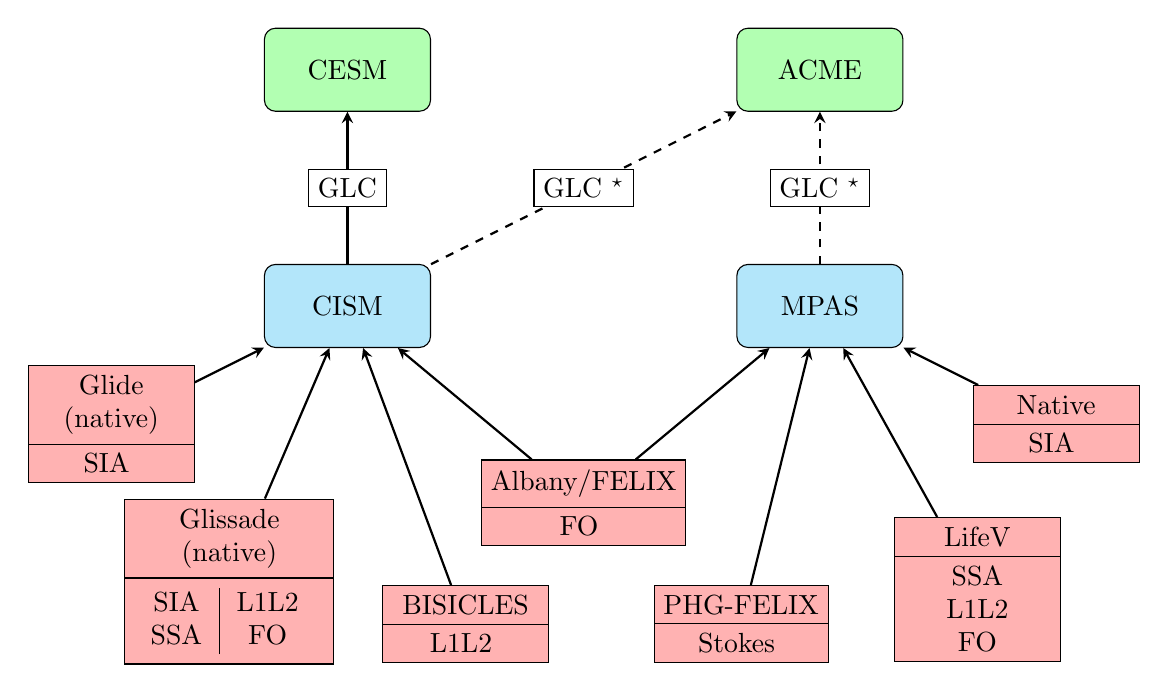
\begin{tikzpicture}[scale=2]
            \node [climateModel] (CESM) {CESM};
\node [climateModel] (ACME)   at ([shift={(3,0)}] CESM) {ACME};

\node [iceModel] (CISM)       at ([shift={(0,-1.5)}] CESM) {CISM};
\node [iceModel] (MPAS)       at ([shift={(0,-1.5)}] ACME) {MPAS};


\node [dycore] (Glide)        at ([shift={(-1.5,-.75)}] CISM) {
    Glide \\ (native)
    \nodepart{second} SIA
    };
\node [dycore] (Glissade)     at ([shift={(-.75,-1.75)}] CISM) {
    Glissade \\ (native)
    \nodepart{second} 
    \begin{tabular}{c|c}
        SIA & L1L2 \\ 
        SSA & FO 
    \end{tabular}
    };
\node [dycore] (BISICLES)     at ([shift={(.75,-2.02)}] CISM) {
    BISICLES
    \nodepart{second} L1L2 
    };
\node [dycore] (Albany) at ([shift={(1.5,-1.25)}] CISM) {
    Albany/FELIX
    \nodepart{second} FO
    };


\node [dycore] (PHG)    at ([shift={(-.5,-2.02)}] MPAS) {
    PHG-FELIX 
    \nodepart{second} Stokes
    };
\node [dycore] (LifeV)        at ([shift={(1,-1.8)}] MPAS) {
    LifeV
    \nodepart{second} SSA \\ L1L2 \\ FO
    };
\node [dycore] (Native)       at ([shift={(1.5,-.75)}] MPAS) {
    Native
    \nodepart{second} SIA
    };


\draw [arrow] (CISM) -- (CESM);
\draw [dashedArrow] (CISM) -- (ACME);
\draw [dashedArrow] (MPAS) -- (ACME);

\draw [arrow] (Glissade) -- (CISM);
\draw [arrow] (Glide) -- (CISM);
\draw [arrow] (Albany) -- (CISM);
\draw [arrow] (BISICLES) -- (CISM);

\draw [arrow] (Albany) -- (MPAS);
\draw [arrow] (PHG) -- (MPAS);
\draw [arrow] (LifeV) -- (MPAS);
\draw [arrow] (Native) -- (MPAS);

\node [textBox] at ([shift={(0,-.75)}] CESM) {GLC}; 
\node [textBox] at ([shift={(1.5,-.75)}] CESM) {GLC $^{\star}$};
\node [textBox] at ([shift={(3,-.75)}] CESM) {GLC $^{\star}$};


        \end{tikzpicture}
    \end{figure}

    \vspace{3em}
    $\star \;$ Generalize, split up, ... move glint into the coupler to pass fields

    \vspace{1em}
    Notes:
    
    \vspace{.5em}
    Glide solves the SIA thickness evolution directly while the Glissade-SIA 
    calculates a local SIA velocity and then does standard advection with it.
\end{document}
